
Using a test data set, we tested the LOFAR \texttt{prefactor} target pipeline on the SURFsara \texttt{GINA} cluster. First we will present the tests done in an isolated environment and then compare them to the run time in production on a shared infrastructure. We will integrate all the results in a complete model which can be used to predict processing time for a variety of parameters. Finally, we will make some predictions on the run time of our processing based on the model and validate these predictions. 

Since we are  processing a sample data set in the context of the LOFAR Surveys project, we will compare these tests with the production runs of our pipeline. In production, we run  the {\fontfamily{qcr}\selectfont gsmcal\_solve} step with a data size of 1GB, a sky model with 180 sources and 8 CPUs. 
 

\subsection{Isolated Environment tests}
We first tested the LOFAR software in isolation in order to determine the scalability of processing time in terms of data size. We run the entire \texttt{prefactor} target pipeline which which removes Direction Independent Calibration errors from a LOFAR science target. In the following sections, we present the models obtained from these tests.  

\subsubsection{Input Data Size}\label{sec:ch6_results_size}
LOFAR data can be averaged to different sizes based on the scientific requirements. Smaller data sets are processed faster, so it is important to understand the effect of data size on processing time as measured by wall-clock time. We show the processing time for our test data set, averaged to different sizes for several \texttt{prefactor} steps in Figures \ref{fig:ch6_predict_ateam}- \ref{fig:ch6_gsmcalsolve_size} and \ref{fig:ch6_gsmcalapply_size}. We run this test using 8 CPUs. The figures also show linear fits for consecutive pairs of parameter steps, in gray dashed lines, used to help guide the selection of parametric model. 

All of the steps show a linear behavior with respect to input data size, while the {\fontfamily{qcr}\selectfont gsmcal\_solve step} is best fit by two linear relationships, for data smaller and larger than 16 GB. The linear fit to the run times are shown in Equations \ref{eq:ch6_predictateam}-\ref{eq:ch6_gsmcalapply}. The equations show the processing time as a function of the data size ($\mathcal{S}$), with the slope in the units of seconds/byte. The fits are also shown in Figures \ref{fig:ch6_predict_ateam} to \ref{fig:ch6_gsmcalapply_size} as a black dashed line.

\begin{equ*}
\begin{subequations}
\begin{align}
        T_{predict\_ateam}=5.19\times10^{-8}\mathcal{S}+4.20\times10^1 \label{eq:ch6_predictateam} \\
        T_{ateamcliptar}=4.57\times10^{-9}\mathcal{S}-8.42\times10^0 \label{eq:ch6_ateamcliptar} \\
        T_{dpppconcat}=3.51\times10^{-8}\mathcal{S}+4.20\times10^1 \label{eq:ch6_dpppconcat} \\
        T_{gsmcal\_solve}=\begin{cases}
                          7.38\times10^{-7}\mathcal{S}-8.20\times10^1 &|\mathcal{S}\leq1.6\times10^{10}\\
                          1.04\times10^{-6}\mathcal{S}-4.04\times10^3 & |\mathcal{S}>1.6\times10^{10}
    \end{cases} \label{eq:ch6_gsmcalsolve} \\
        T_{gsmcal\_apply}=2.07\times10^{-8}\mathcal{S}-1.38\times10^1 \label{eq:ch6_gsmcalapply}    
\end{align}
\label{eq:ch6_runtime_size_models}
\end{subequations}
\caption{Equations describing the processing time of five \texttt{prefactor} steps as a function of the input data size ($\mathcal{S}$) in bytes.}
\end{equ*}


\begin{figure*}[t!]
        \centering
        \begin{subfigure}[b]{0.44\textwidth}
            \centering
            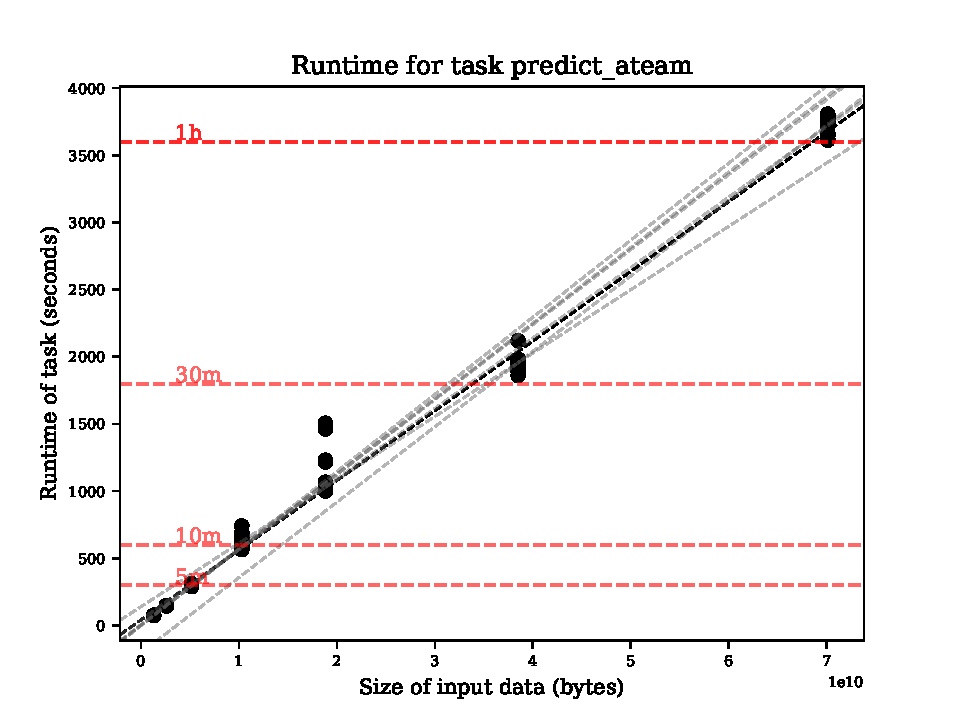
\includegraphics[width=\textwidth]{ch6/figures/predict_ateam_size.pdf}
            \caption[]%
            {{\small Tests of the  {\fontfamily{qcr}\selectfont predict\_ateam} step for input data size ranging from 1GB to 64 GB. This step calculates the contamination from bright off-axis sources. Dashed lines are shown connecting each pair of points, to highlight the trend. We can see that the data can be described well by a linear model. We show the model in Equation \ref{eq:ch6_predictateam} in black.}}   
            \label{fig:ch6_predict_ateam}
        \end{subfigure}
        \hfill
        \begin{subfigure}[b]{0.44\textwidth}  
            \centering 
            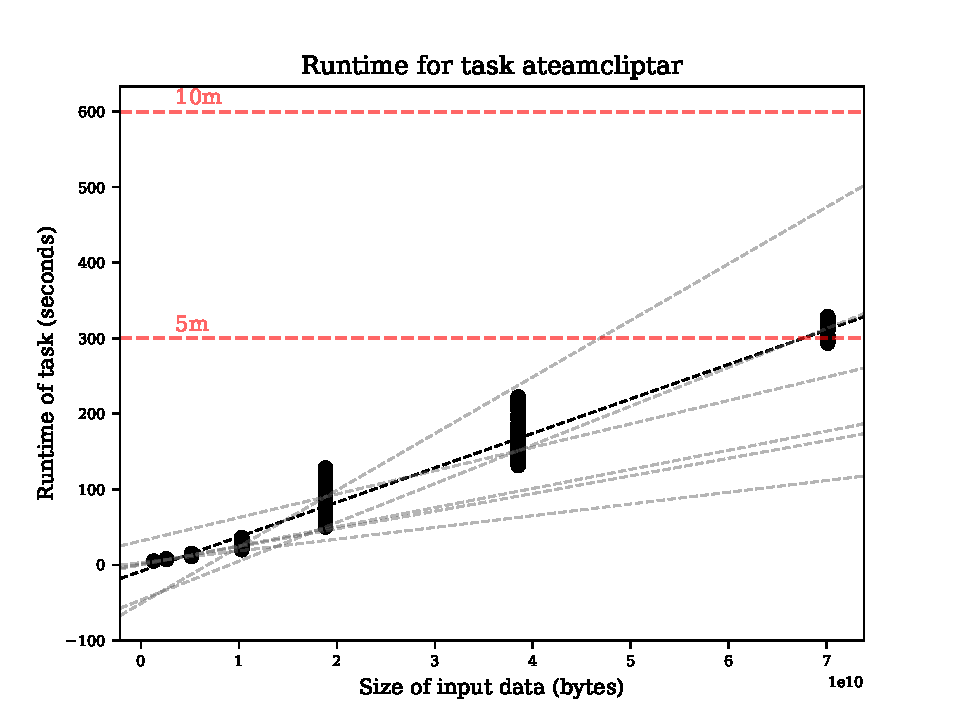
\includegraphics[width=\textwidth]{ch6/figures/ateamcliptar_size.pdf}
            \caption[]%
            {{\small Tests of the {\fontfamily{qcr}\selectfont ateamcliptar} step for input data size ranging from 1GB to 64 GB. This step removes the contamination from bright off-axis sources. We can see that the data fits a linear model. We show the model in Equation \ref{eq:ch6_ateamcliptar} in black.}}    
            \label{fig:ch6_ateamcliptar}
            \end{subfigure}
        \vskip\baselineskip
        \begin{subfigure}[b]{0.44\textwidth}   
            \centering 
            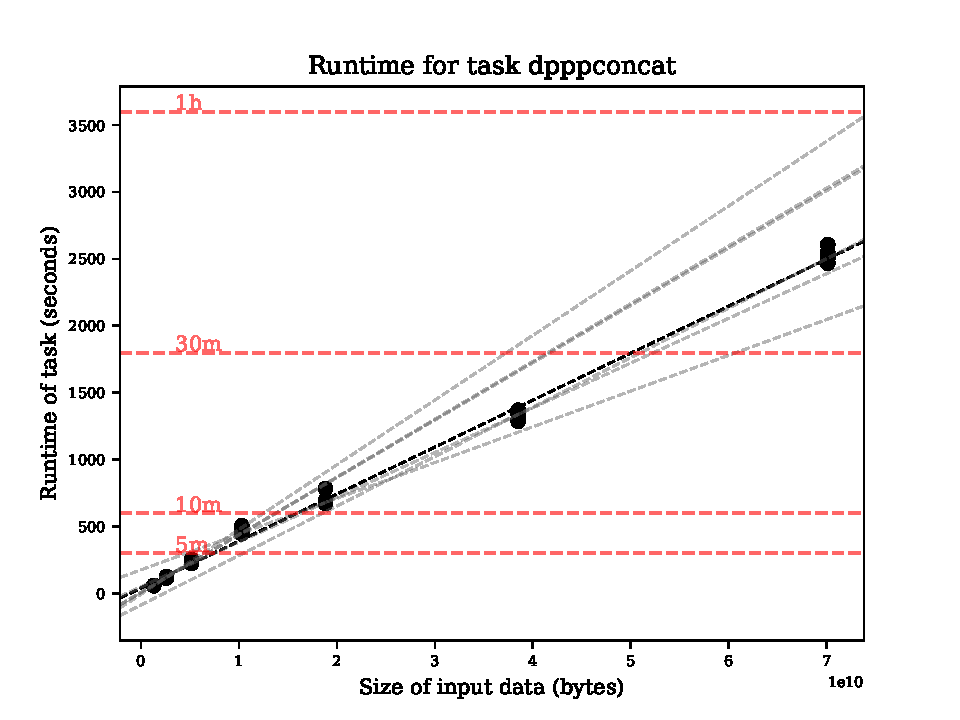
\includegraphics[width=\textwidth]{ch6/figures/dpppconcat_size.pdf}
            \caption[]%
            {{\small Tests of the {\fontfamily{qcr}\selectfont dpppconcat} step for input data size ranging from 1GB to 64 GB. This step concatenates 10 files into a single measurement set.  We can see that the data fits a linear model. We show the model in Equation \ref{eq:ch6_dpppconcat}  in black.}}    
            \label{fig:ch6_dpppconcat_size}
        \end{subfigure}
        \hfill
        \begin{subfigure}[b]{0.44\textwidth}   
            \centering 
            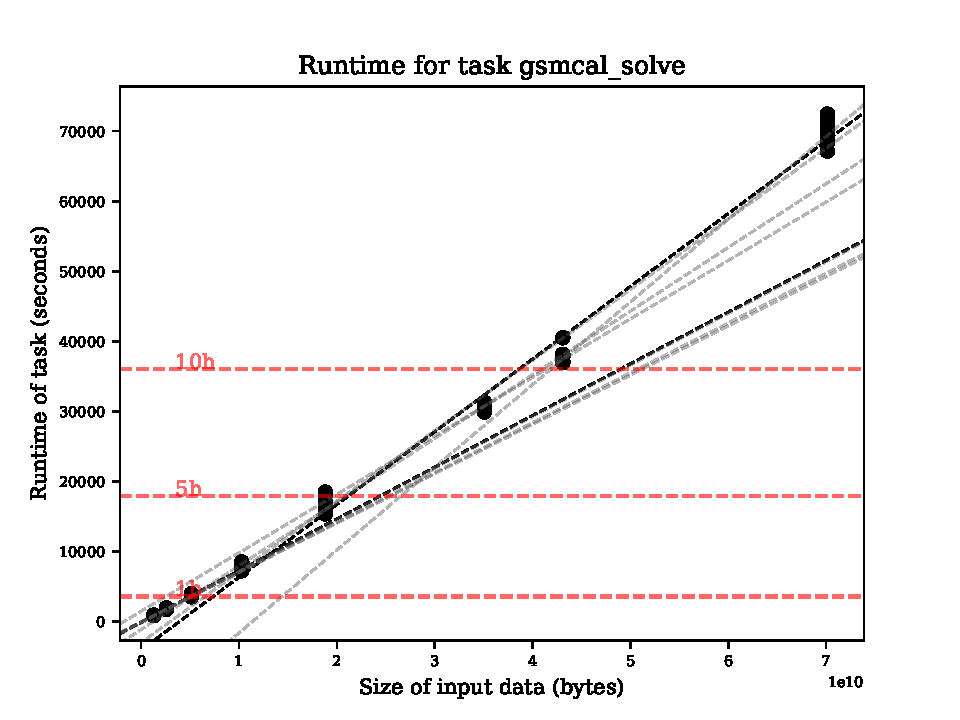
\includegraphics[width=\textwidth]{ch6/figures/gsmcal_solve_size2.pdf}
            \caption[]%
            {{\small Tests of the {\fontfamily{qcr}\selectfont gsmcal\_solve} step for input data size ranging from 1GB to 64 GB. This step performs gain calibration of the concatenated data set against a sky model. It is the slowest and most computationally expensive \texttt{prefactor} step. We fit two linear models, for data below 16GB and above 16GB. We can see the two models, shown in  (Equation \ref{eq:ch6_gsmcalsolve}) as two black dashed lines, intersecting at 1GB.}}    
            \label{fig:ch6_gsmcalsolve_size}
        \end{subfigure}
        \caption[ ]
        {\small Plots of the run time as a function of input data size} 
\end{figure*}


\begin{figure}
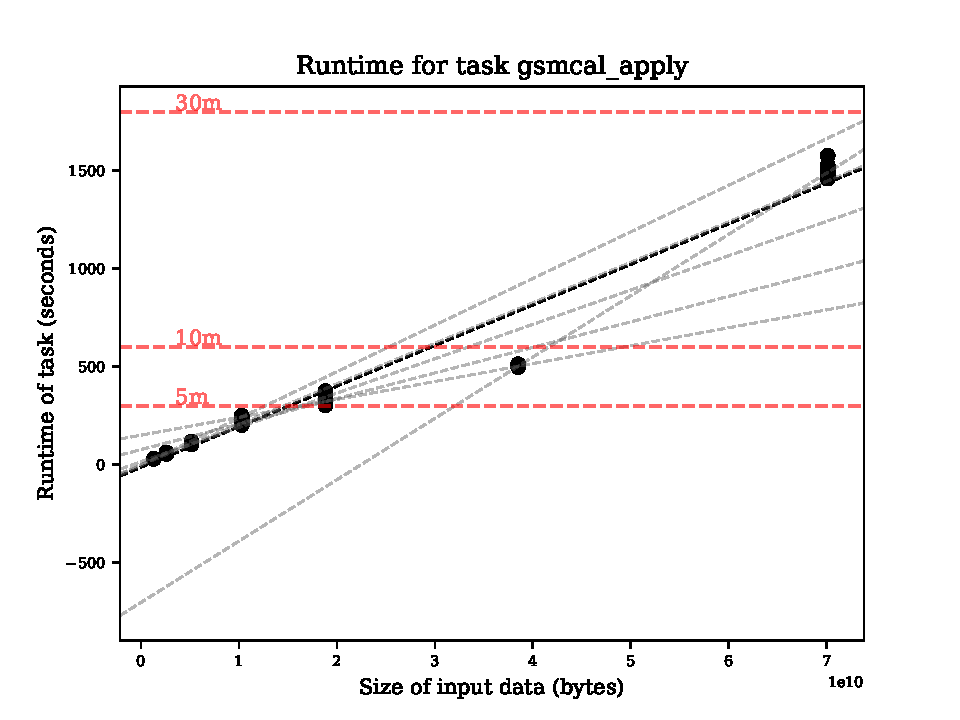
\includegraphics[width=0.95\linewidth]{ch6/figures/gsmcal_apply_size.pdf}
        \caption{\small Tests of the {\fontfamily{qcr}\selectfont gsmcal\_apply} step for input data size ranging from 1GB to 64 GB. This step applies the calibration solutions to the data. We can see that the data fits a linear model, described in Equation\ref{eq:ch6_gsmcalapply}, as the black dashed line.}
            \label{fig:ch6_gsmcalapply_size}
\end{figure}

\subsubsection{Calibration Model Size}
To test the effect of the calibration model size on run time, we test our calibration with several different lengths of the sky model file. We create these models by changing the minimum sensitivity using values ranging from 0.05 Jy to 1.5 Jy. The most sensitive model (0.05 Jy) had 809 sources while the 1.5 Jy model had only 16 sources. 

Figure \ref{fig:ch6_skymodel_run_lenght} shows that the calibration time is directly proportional to the length of the sky model. Figure \ref{fig:ch6_skymodel_run_sens} shows the run time as a function of the processing parameter: the cutoff sensitivity. As the relationship between the number of sources and cutoff sensitivity is a power law, here we see the same relationship holding for processing time.

We model the processing time as a function of the cutoff frequency using a power law, and fit the data to the function $y=\alpha\cdot \mathcal{F}^{-k}$. Our fit found the best model to be shown in Equation \ref{eq:ch6_skymodel_flux}, where $\mathcal{F}$ value is the cutoff flux in Jansky and $T$ is the run time in seconds. 

We show four images made from data sets in Figure \ref{fig:ch6_skymodel_images}. The top left image is calibrated with a 0.05Jy and the other three show the difference between the top left image and the images created from the 0.3Jy, 0.8 Jy and 1.5 Jy data. The statistics for the four images, taken from the regions in green on Figure \ref{fig:ch6_skymodel_images}) are shown in Table \ref{table:skymodel_RMS}. We discuss the implication and caveats of these results in Section \ref{sec:ch6_discussions}.


\begin{table}[h!]
\centering
\begin{tabular}{||p{2.8cm}| c | c ||} 
 \hline
 Calibration Model Flux Cutoff & \# of sources& RMS Noise (Jy) \\ %%& std dev (Jy) \\ [0.5ex]
 \hline
 0.05Jy & 809 &0.00402834   \\ %& 0.004026    \\ 
  \rowcolor{Gray}
  \hline
 0.3 Jy & 180 &0.00402311 \\ %& 0.004020 \\
 \hline
 0.8 Jy & 49 &0.00404181 \\ %& 0.004039 \\  
 1.5 Jy & 16 &0.00410204 \\ %& 0.004105\\
 \hline
\end{tabular}
    \caption[Image statistics for four different sky models]{Statistics for an empty region for the four images shown in Figure \ref{fig:ch6_skymodel_images}. The 0.3Jy model, here shown shaded in gray,  is the one used in production.  }
\label{table:skymodel_RMS}
\end{table}

\begin{equ}
\begin{equation}
    T=1185\cdot \mathcal{F}^{-0.854}
\label{eq:ch6_skymodel_flux}
\end{equation}
\caption{Processing time for the {\fontfamily{qcr}\selectfont gsmcal\_solve} step as a function of the flux cutoff of the calibration model ($\mathcal{F}$) in Jansky}
\end{equ}

\begin{figure}
    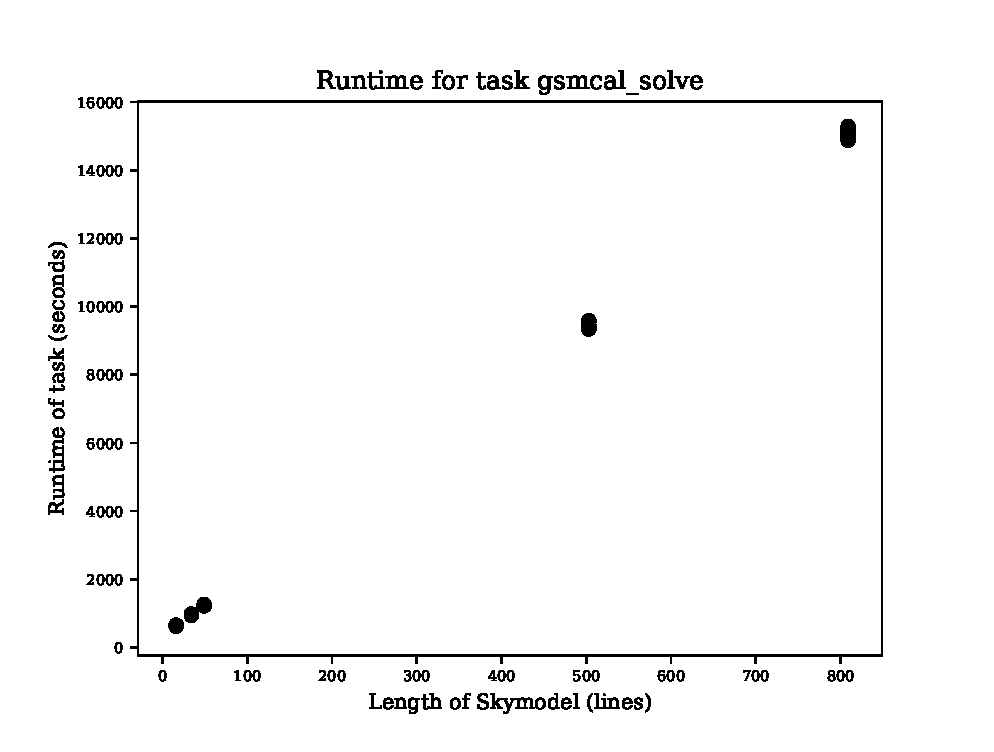
\includegraphics[width=0.95\linewidth]{ch6/figures/skymodel_length.eps}
      \caption{The processing time of the {\fontfamily{qcr}\selectfont gsmcal\_solve} step is linear with the size of the sky model as measured by the number of sources.}
	\label{fig:ch6_skymodel_run_lenght}
\end{figure}

\begin{figure}
    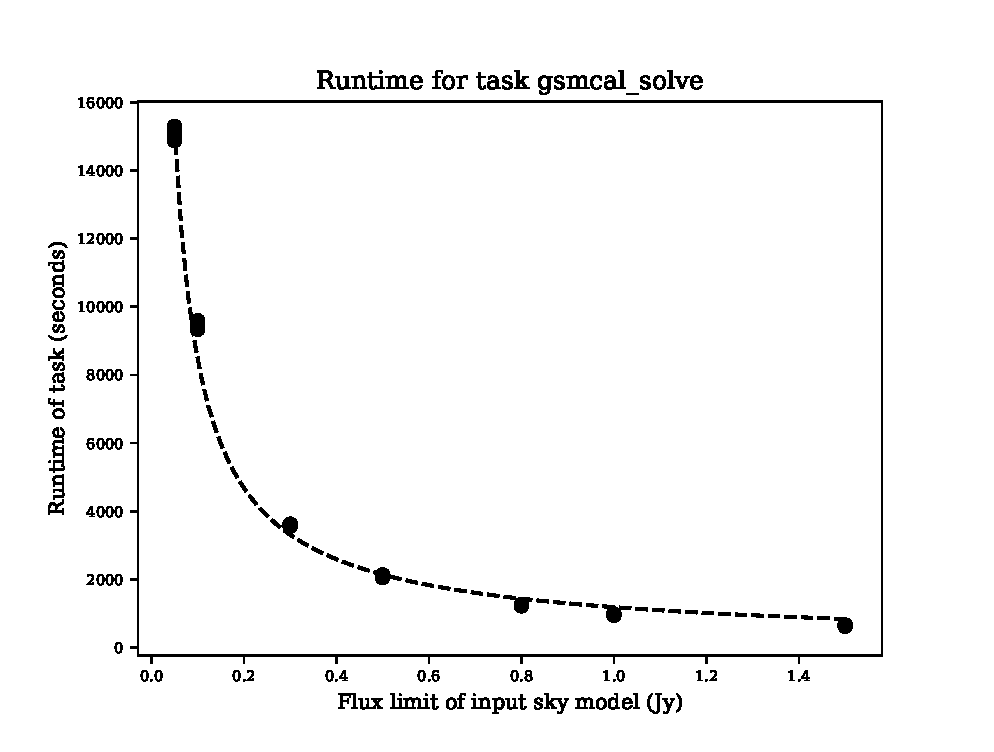
\includegraphics[width=0.95\linewidth]{ch6/figures/skymodel_flux.eps}
      \caption{The run time of the {\fontfamily{qcr}\selectfont gsmcal\_solve} step as a function of the cutoff sensitivity is not linear. As shown in Figure \ref{fig:ch6_skymodel_size}, the number of sources increases exponentially as the minimum sensitivity decreases. The dashed line shows the model fitted in Equation \ref{eq:ch6_skymodel_flux}. }
	\label{fig:ch6_skymodel_run_sens}
\end{figure}

\begin{figure*}
    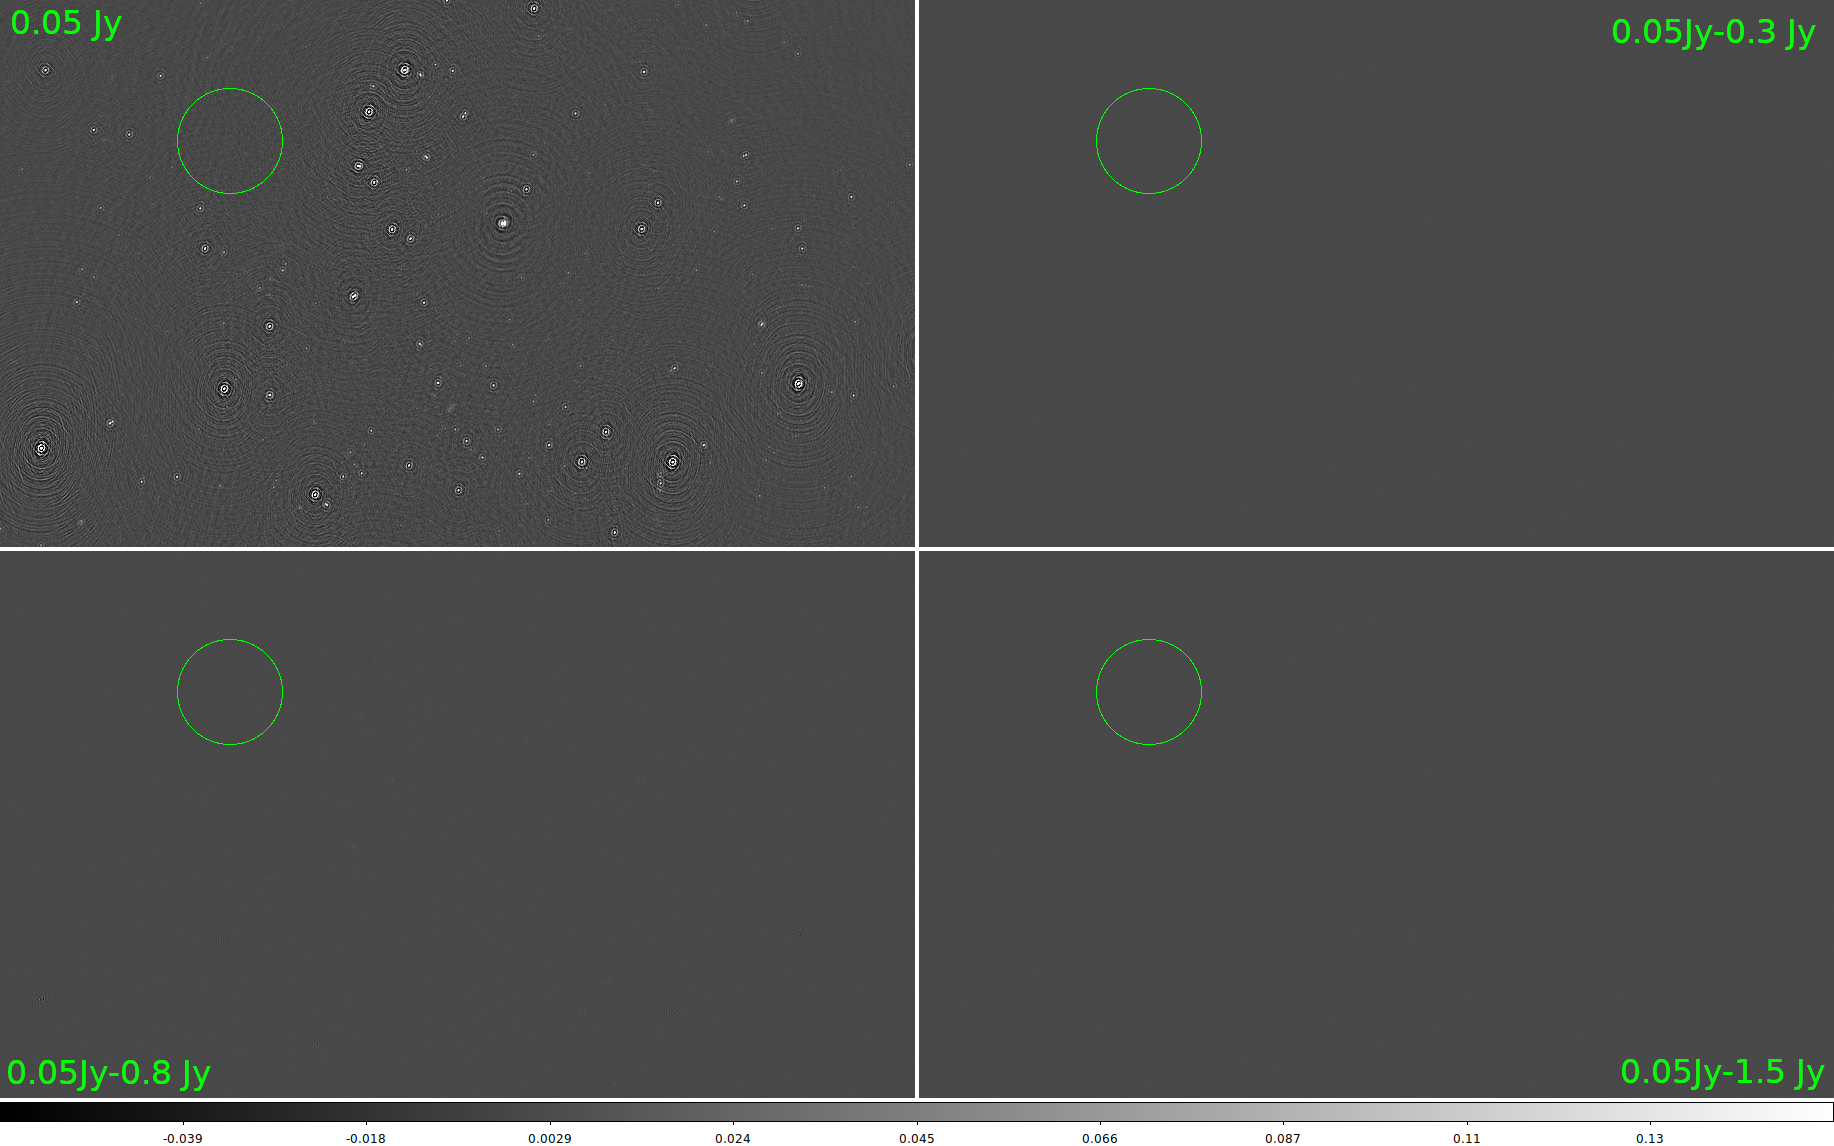
\includegraphics[width=0.95\linewidth]{ch6/figures/difference_4.png}
      \caption{Four images made using the \texttt{wsclean} software \citep{wsclean} from the data set\protect\footnotemark. The four images were calibrated with sky models of various flux cutoffs ranging from 0.05Jy (top left) to 1.5Jy (bottom right). Flux statistics for the green regions in the four images are listed in Table \ref{table:skymodel_RMS}. The top right, and bottom two quadrants show the pixel difference between the 0.05Jy image and the 0.3Jy, 0.8Jy and 1.5Jy images respectively. The four images are all on the same scaleThe green region shows the same area in all four quadrants.  }
	\label{fig:ch6_skymodel_images}
\end{figure*}
\footnotetext{Using the command wsclean -absmem 50 -niter 3 -size 4096 4096 -scale 20asec}



\subsubsection{Number of CPUs}
One further parameter that can be optimized is the number of CPUs requested when the job is launched. We investigated the processing speedup as a function of the number of CPUs for the \texttt{prefactor} target pipeline. From the steps tested, only the {\fontfamily{qcr}\selectfont gsmcal\_solve} step shows a significant speedup as the number of CPUs is increased. The run time of this step is an inverse power law with respect to the number of CPUs as seen in Figure \ref{fig:ch6_gsmcal_solve_NCPU}. Unlike the solving step, the step applying the calibration solutions ({\fontfamily{qcr}\selectfont gsmcal\_apply}) is constant in time with respect to the number of CPUs as seen in Figure \ref{fig:ch6_gsmcal_apply_NCPU}. The difference in performance is most likely because the {\fontfamily{qcr}\selectfont gsmcal\_apply} code uses a parallel for loop to calculate antenna gains while {\fontfamily{qcr}\selectfont gsmcal\_apply} does not. 

We fit a model with processing time inversely proportional to the number of CPUs used. We show the resulting model in Equation \ref{eq:ch6_gsmcal_NCPU}, with the parameter $(\mathcal{N})$ being the number of CPUs used. 

\begin{figure}
    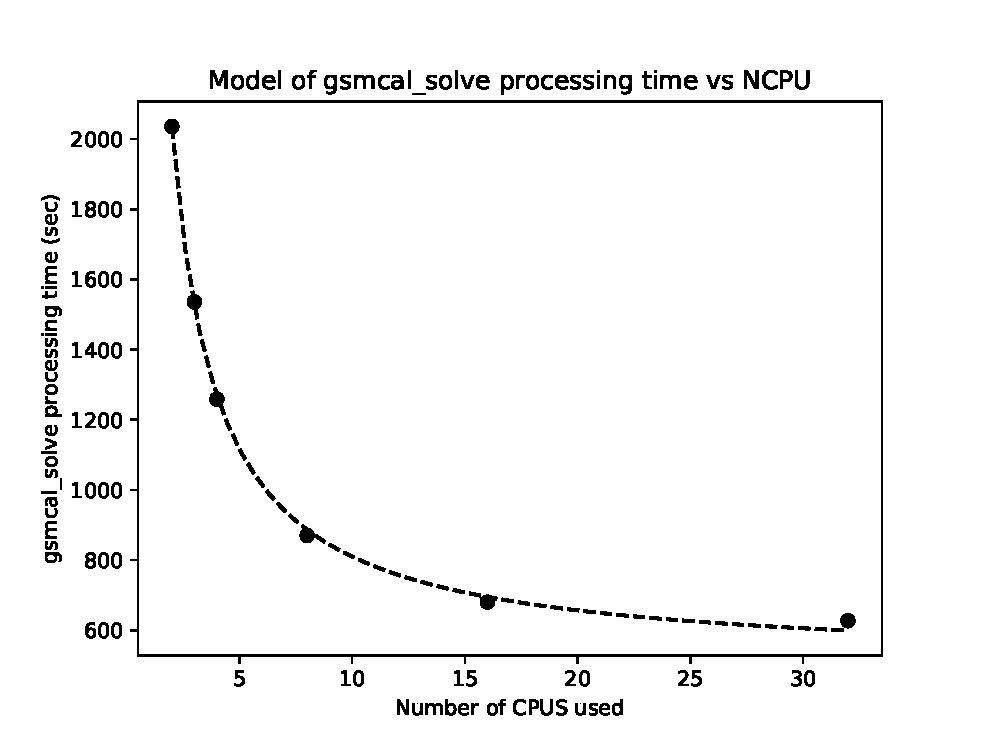
\includegraphics[width=0.95\linewidth]{ch6/figures/gsmcal_NCPU_and_model.eps}
      \caption{The processing time of the {\fontfamily{qcr}\selectfont gsmcal\_solve} step decreases exponentially with the number of CPUs requested. The model in Equation \ref{eq:ch6_gsmcal_NCPU} is shown in a dashed line. As this is a 1/x model, it shows diminishing returns past 16 CPUs. }
	\label{fig:ch6_gsmcal_solve_NCPU}
\end{figure}

\begin{figure}
    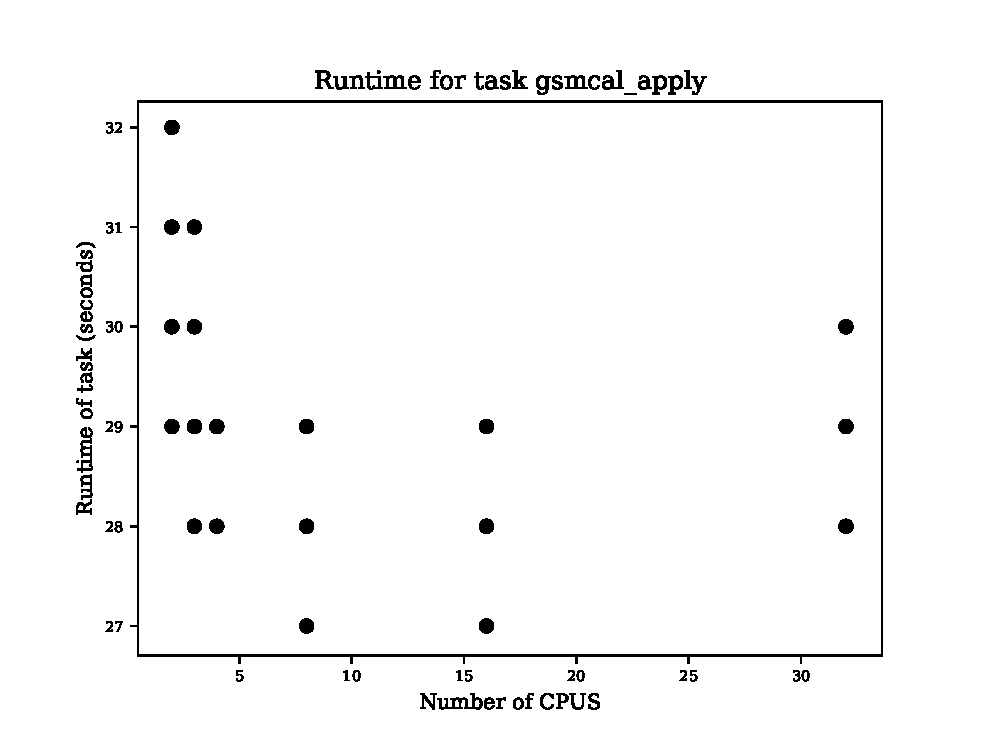
\includegraphics[width=0.95\linewidth]{ch6/figures/gsmcal_apply_NCPU.eps}
      \caption{The step that applies the calibration solutions, {\fontfamily{qcr}\selectfont gsmcal\_apply}, does not show a speedup when run on multiple cores, as all runs take roughly 30 seconds to complete.  }
	\label{fig:ch6_gsmcal_apply_NCPU}
\end{figure}

\begin{equ}
\begin{equation}
    T=503.37+\frac{3062.6}{\mathcal{N}}
\label{eq:ch6_gsmcal_NCPU}
\end{equation}
\caption{Processing time for the {\fontfamily{qcr}\selectfont gsmcal\_solve} step as a function of ($\mathcal{N}$), the Number of CPUs used by the process.}
\end{equ}


\subsection{Queuing Tests}

Aside from performance of the LOFAR software, we measured the queuing time at the \texttt{GINA} cluster, as a function of the number of CPUs requested. This data was obtained between 16 Nov 2018 and 10 Dec 2018 for 1,  2, 3 ,4, 8, and 16 CPUs per job. A histogram of the queuing time for these jobs is shown in Figure \ref{fig:ch6_queue_NCPU}. Statistics for these runs are in Table \ref{table:queueing_stats}. We use the 75th percentile of the queuing time for each parameter step to fit a model. This scenario will include 75\% of runs and is a good trade-off between ignoring and including outliers. 

We fit two linear models for this queuing time. One model for 1-4 CPUs and one for 4-16 CPUs. The model, as a function of the number of CPUs $\mathcal{N}$ is in equation \ref{eq:ch6_queue_model}. The two models are plotted against the 75th percentile of the queuing times (last column in Table \ref{table:queueing_stats}) in Figure \ref{fig:ch6_queue_model}.

\begin{figure}
    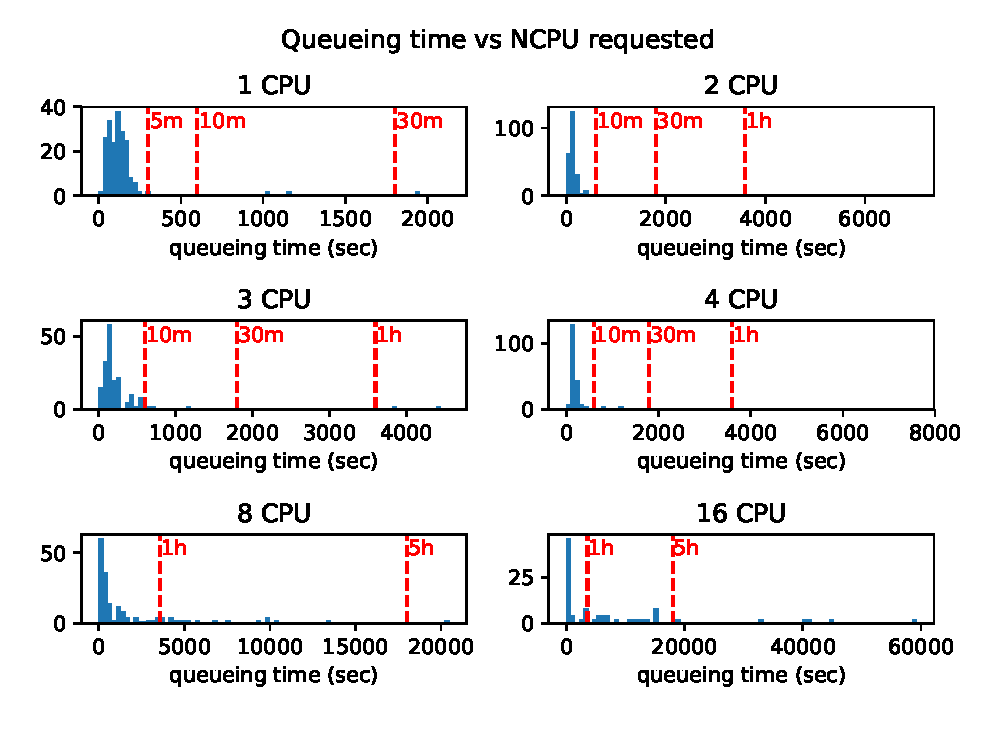
\includegraphics[width=0.95\linewidth]{ch6/figures/Queue_NCPU.eps}
      \caption{Test randomly submitting jobs to the \texttt{GINA} with different number of requested CPUs. The long tail for 8 and 16 CPU jobs shows that some jobs can take several hours to launch.  }
      
      %Outliers due to grid downtime have been removed \textbf{Actually do this though} }
	\label{fig:ch6_queue_NCPU}
\end{figure}


\begin{table*}[t]
\centering
\begin{tabular}{||p{2.8cm}|c | c | c||} 
 \hline
 NCPU requested & Mean time (sec) & Median time (sec) & 75th percentile (sec)\\ [0.5ex]
 \hline
 1 CPU & 150.5   & 116.2 & 154.1   \\ 
 2 CPU & 201.1 & 125.8 & 165.8 \\
 3 CPU & 296.2 & 152.0 & 243.0 \\
 4 CPU & 498.9 & 167.7 & 233.7\\
 8 CPU & 1944.2 & 428.4 & 2142.4\\
 16 CPU & 7079.0 & 696.4 & 8750.6\\
 \hline
\end{tabular}
    \caption[Queueing statistics per requested number of CPUs]{Statistics for queuing time for different values of CPUs requested. Queuing time for jobs requesting less than 8 CPUs is typically less than five minutes. It can drastically increase for larger jobs. }
\label{table:queueing_stats}
\end{table*}

\begin{figure}
    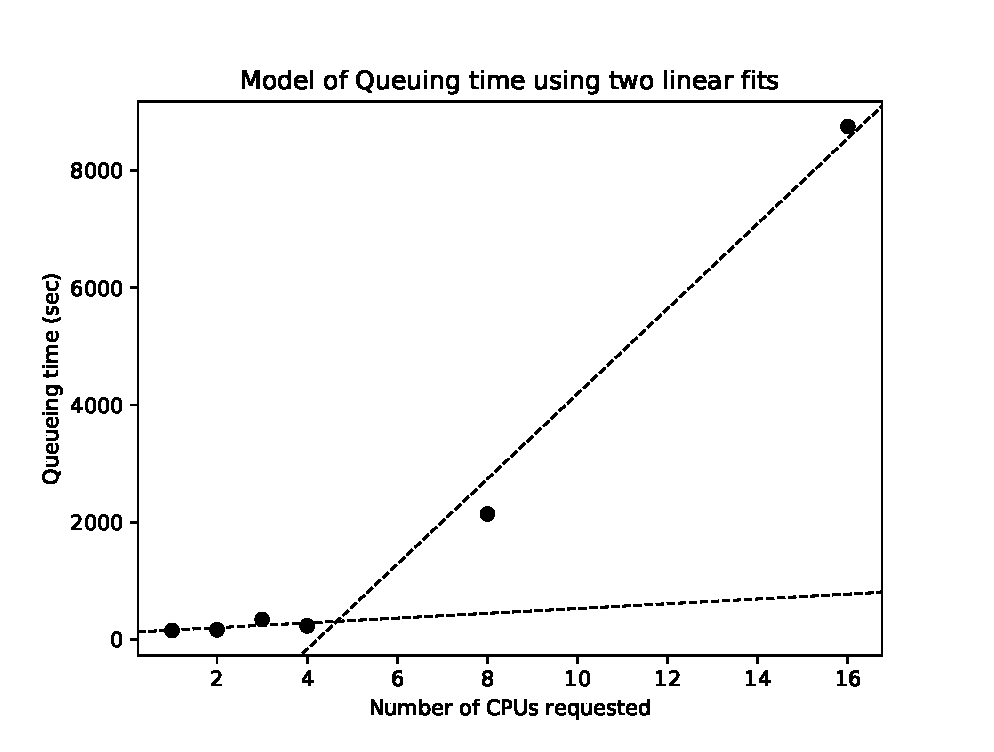
\includegraphics[width=0.95\linewidth]{ch6/figures/Queueing_model.eps}
      \caption{The queuing model built from two linear fits to the queuing times. We use the 75th percentile of the queuing data as a upper bound of job queuing. }
	\label{fig:ch6_queue_model}
\end{figure}

\begin{equ}
\begin{equation}
  T = \begin{cases}
    49.3\cdot\mathcal{N}+ 120 &|\mathcal{N}\leq4\\
    726\cdot\mathcal{N}-3071 & |\mathcal{N}>4
    \end{cases}
  \label{eq:ch6_queue_model}
\end{equation}
\caption{The model for the Queuing time as described by two linear models. }
\end{equ}



\subsection{Transfer and Unpacking Time}\label{sec:ch6_results_dl}

We tested the downloading and unpacking time for data sizes ranging from 512MB to 64GB. We discovered that the unpacking of files below 64GB scaled linearly with file size, however unpacking individual data sets larger than 16GB becomes considerably slower than downloading it. 

Figure \ref{fig:ch6_dl_hist} shows the histogram of the download tests, and Figure \ref{fig:ch6_dl_plot} displays the tests as a function of data size. Both figures show that extracting of the 32 and 64GB data sets has more slow outliers than the downloading of this data. 

We fit a power law model to the time taken to transfer and unpack the data. In this case, we also consider the 75th percentile of these times in order to capture the majority of runs and ignore outliers. The plot of the data and our model can be seen in Figure \ref{fig:ch6_dl_plot} and the model is in Equation \ref{eq:ch6_download_model}, as a function of the input data size,
$\mathcal{S} $ in gigabytes.

\begin{figure}
    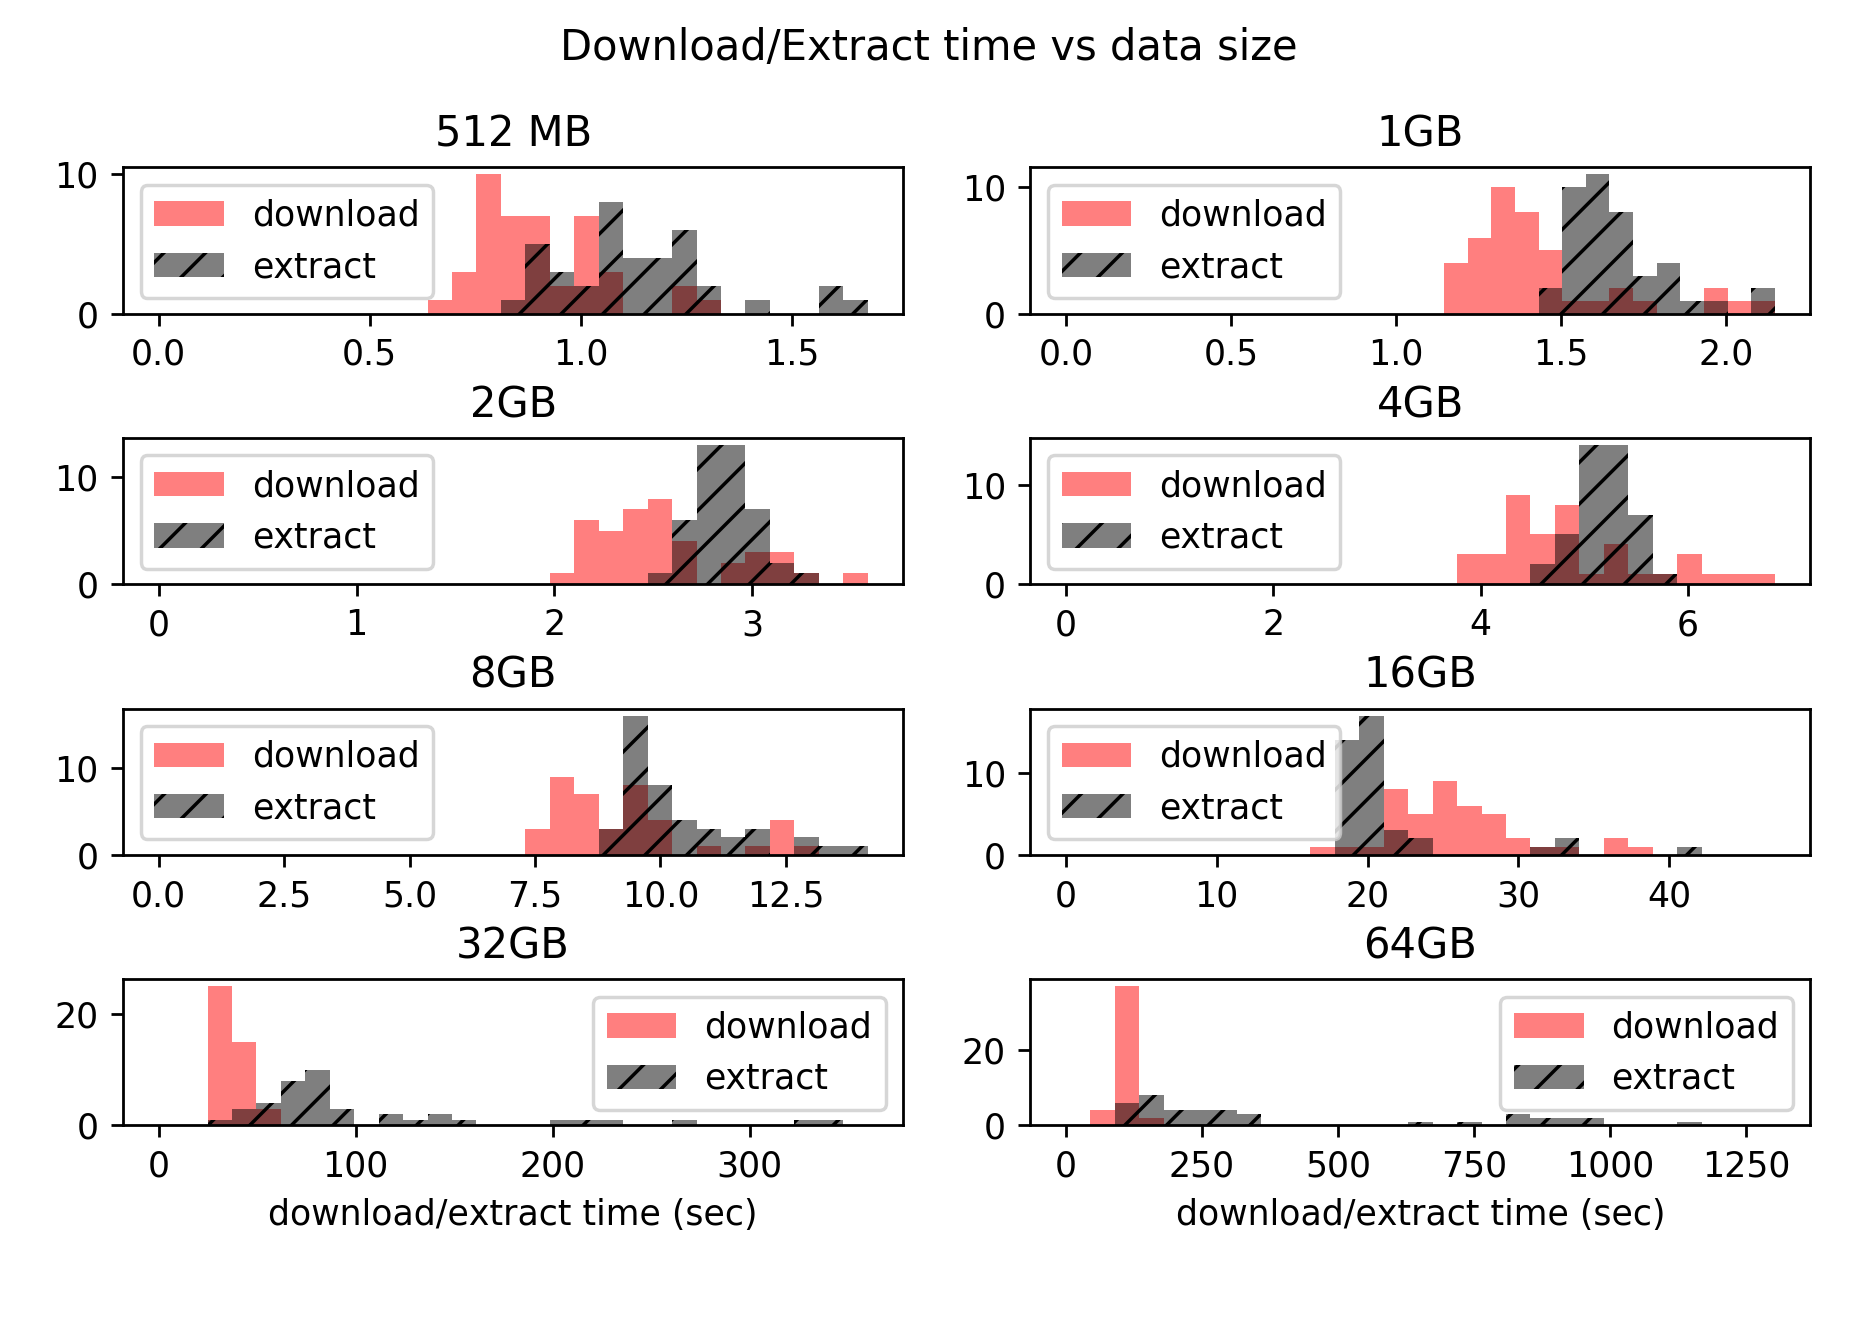
\includegraphics[width=0.95\linewidth]{ch6/figures/dl_ex_hatched.png}
      \caption{A histogram of the download and extracting times of multiple data sizes on the \texttt{GINA} worker nodes. Download and extract times are comparable for data up to 8GB, however above that, the extracting time dominates.  }
	\label{fig:ch6_dl_hist}
\end{figure}

\begin{figure}
    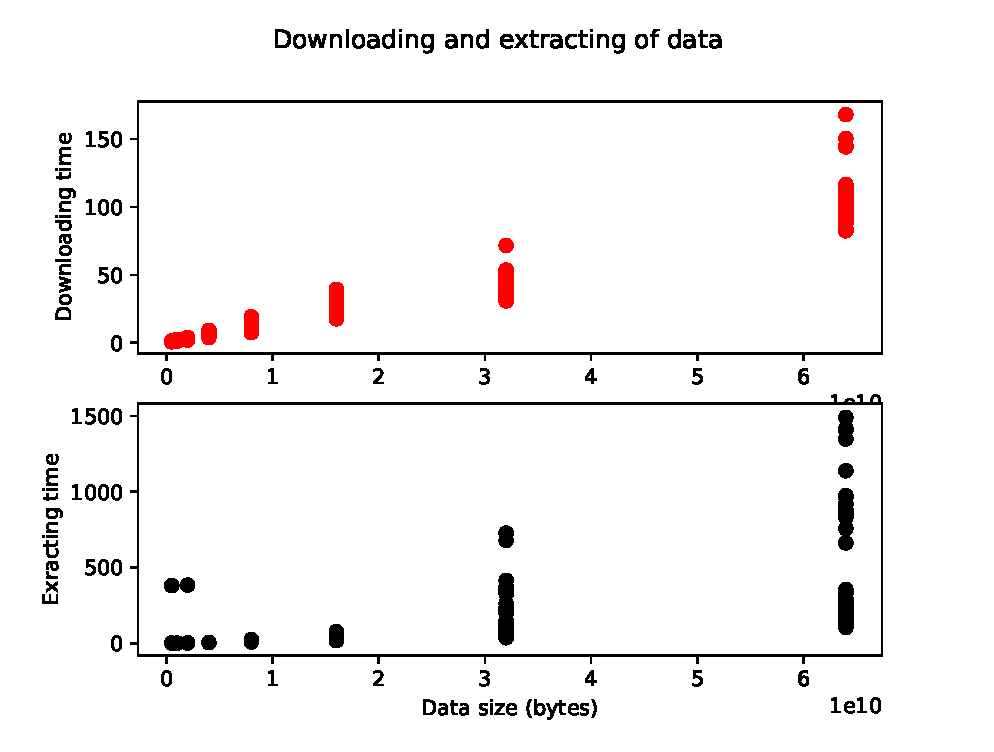
\includegraphics[width=0.95\linewidth]{ch6/figures/download_extract_sct.eps}
      \caption{A scatter plot of the download and extracting times of multiple data sizes on the \texttt{GINA} worker nodes. The difference between download and extract time for the 32 and 64 GB data sets can be seen.  }
	\label{fig:ch6_dl_plot}
\end{figure}

\begin{figure}
    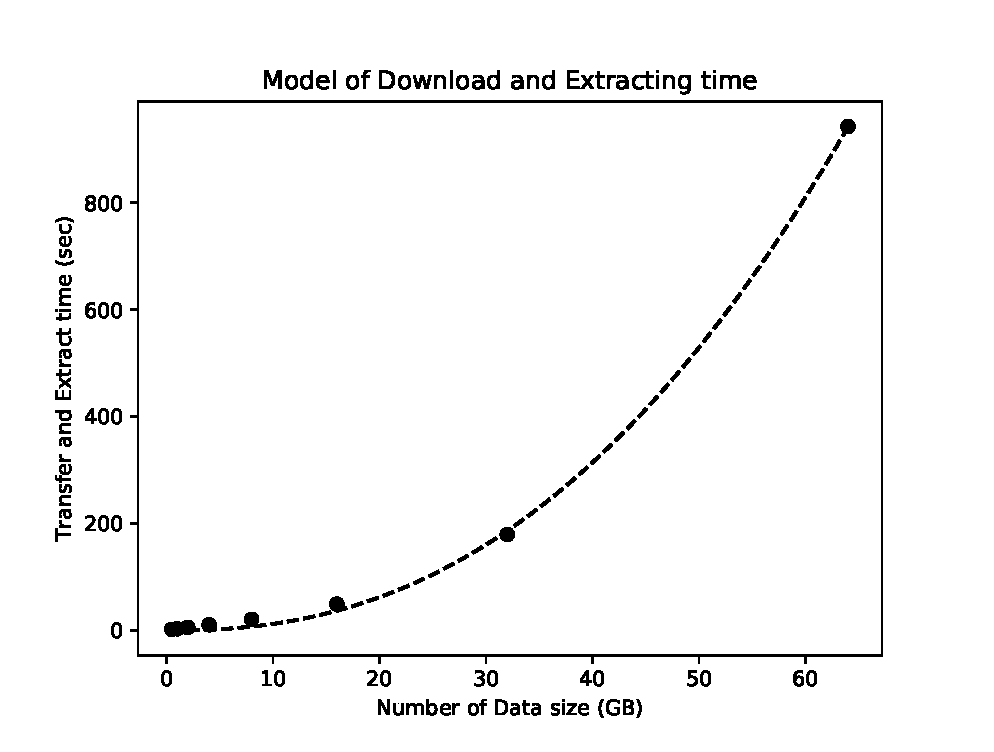
\includegraphics[width=0.95\linewidth]{ch6/figures/Dl_Ex_model.eps}
      \caption{Fit of an exponential model to the Download and Extraction time for different data sizes. For the transfer overhead, we took the 75th percentile from the data shown in Figure \ref{fig:ch6_dl_hist}. The model in Equation \ref{eq:ch6_download_model} is shown in a dashed line. }
	\label{fig:ch6_dl_ex_model}
\end{figure}

\begin{equ}
\begin{equation}
  T=5.918\times10^{20}\cdot \mathcal{S}^{2.336}
  \label{eq:ch6_download_model}
\end{equation}
\caption{Model of the downloading and extracting time as a function of the data size ($\mathcal{S}$) in bytes.}
\end{equ}


\subsection{Comparison with production runs}
Over the past two years, the LOFAR software has been running in production and collecting data on run time for each processing step. We have saved detailed logs for these runs starting in July 2018.  We can compare this to the isolated model in order to determine the overhead incurred by processing LOFAR data on shared nodes. 

Using the logs recorded by our processing launcher \footnote{GRID\_PiCaS\_Launcher, \raggedright\url{https://github.com/apmechev/GRID\_picastools}}, we made plots showing the processing time for the downloading and extracting, and for the slowest steps, {\fontfamily{qcr}\selectfont ndppp\_prepcal} and {\fontfamily{qcr}\selectfont gsmcal\_solve}. 
The results are shown in Figures \ref{fig:ch6_prod_dl_10} and \ref{fig:ch6_prod_dl_64}. We include predicted extract times from Section \ref{sec:ch6_results_dl} as vertical dashed lines for both plots. The agreement between our model and production runs are an encouraging result for future software performance modelling. 

Finally, we present Figure \ref{fig:ch6_prod_gsmcal} which shows a comparison of {\fontfamily{qcr}\selectfont gsmcal\_solve} run times and our model's prediction for a 1GB data set.  Figure \ref{fig:ch6_prod_gsmcal_times} plots the processing time vs data size for these production runs and includes the model from Equation \ref{eq:ch6_gsmcalsolve}. The significant overhead incurred on a shared infrastructure can be noted. 

\begin{figure}
    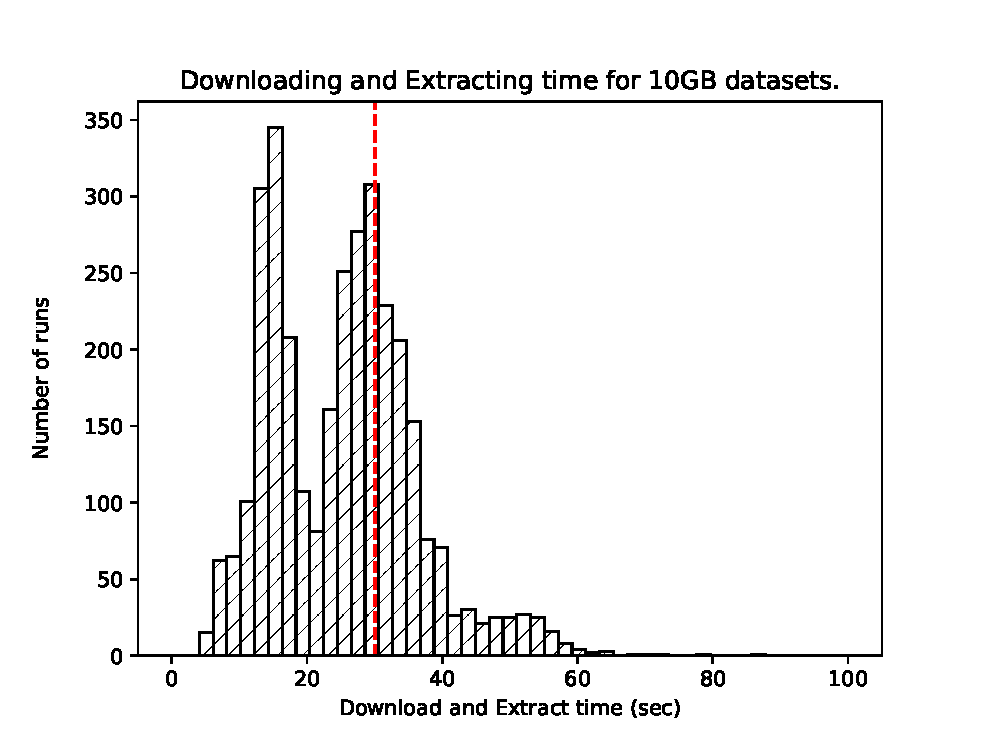
\includegraphics[width=0.95\linewidth]{ch6/figures/Production_10GB_2.eps}
      \caption{Downloading and extracting time for 10 1GB data sets performed in our production environment. Data from this test ranges from July 2018 to January 2019. The dashed red line shows the prediction obtained from section \ref{sec:ch6_results_dl}. We see a bimodal distribution corresponding to 10 GB data (right peak) and data averaged further to 5GB (left peak).}
	\label{fig:ch6_prod_dl_10}
\end{figure}


\begin{figure}
    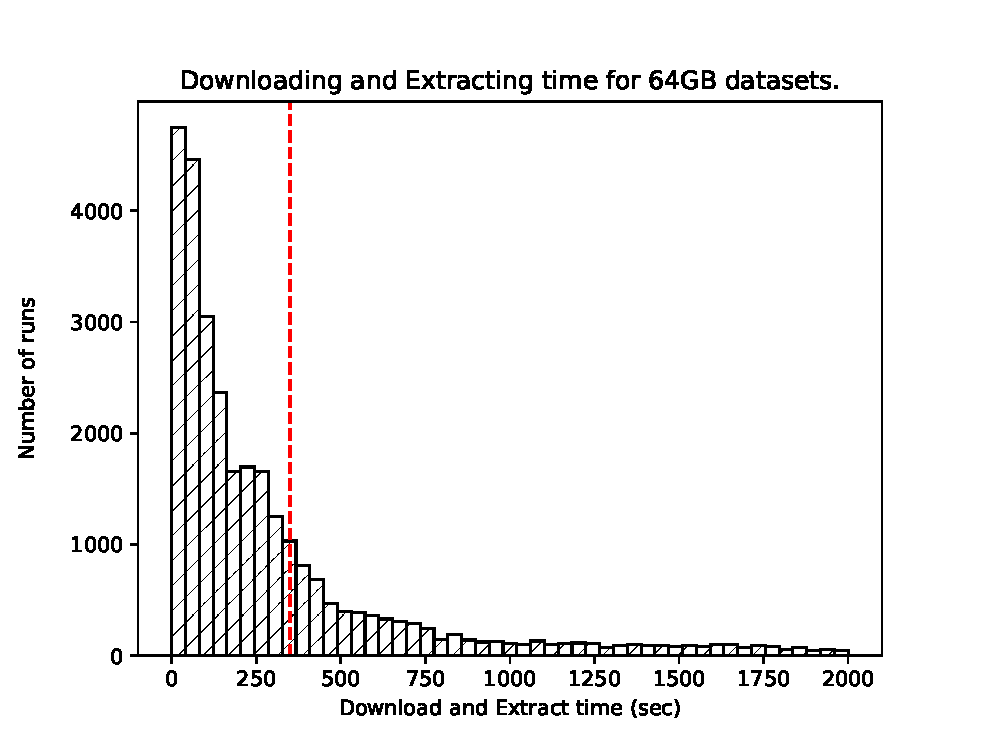
\includegraphics[width=0.95\linewidth]{ch6/figures/Production_64GB_2.eps}
      \caption{Downloading and extracting time for a 64GB data set performed in our production environment. Data from this test ranges from 07/2018-01/2019. The dashed red line shows the prediction obtained from Figure \ref{fig:ch6_gsmcalsolve_size} in Section \ref{sec:ch6_results_dl}. }
	\label{fig:ch6_prod_dl_64}
\end{figure}


\begin{figure}
    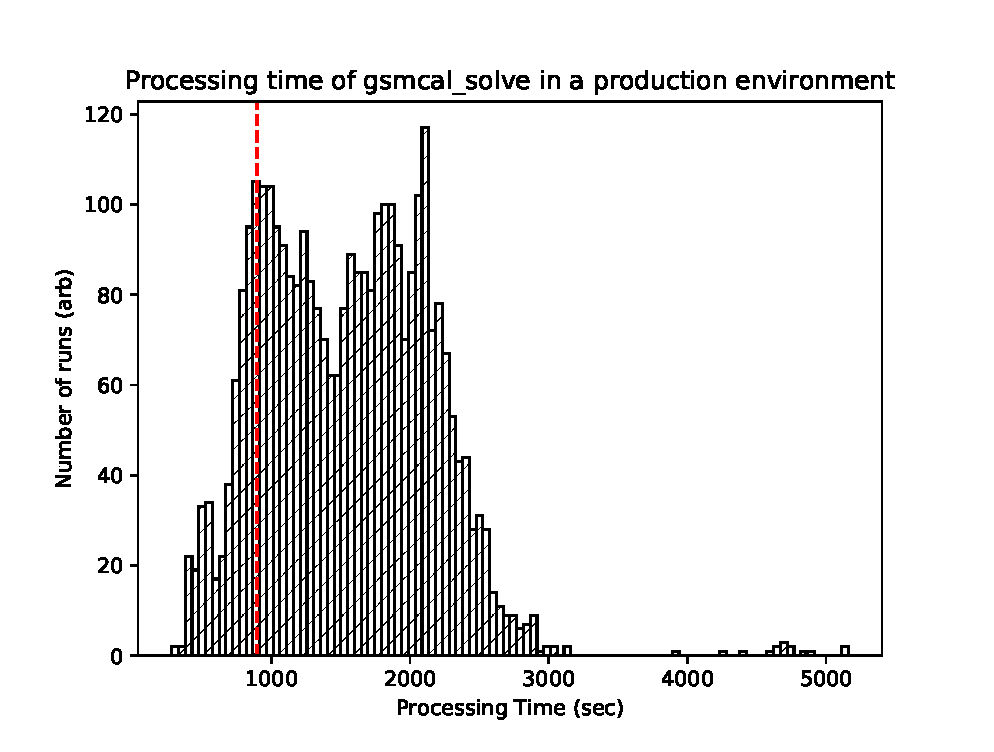
\includegraphics[width=0.95\linewidth]{ch6/figures/Production_gsmcal_1GB_2.eps}
      \caption{Processing time for the {\fontfamily{qcr}\selectfont gsmcal\_solve} step in a production environment. Data from this test ranges from 07/2018-01/2019. The dashed red line shows the prediction for a 1GB run, obtained from section \ref{sec:ch6_results_dl}. We see two distributions, which correspond to data averaged to 1GB and 512 MB.  It should be noted that the left peak corresponds to 512MB data, as seen in Figure \ref{fig:ch6_prod_gsmcal_times}.}
	\label{fig:ch6_prod_gsmcal}
\end{figure}


\begin{figure}
    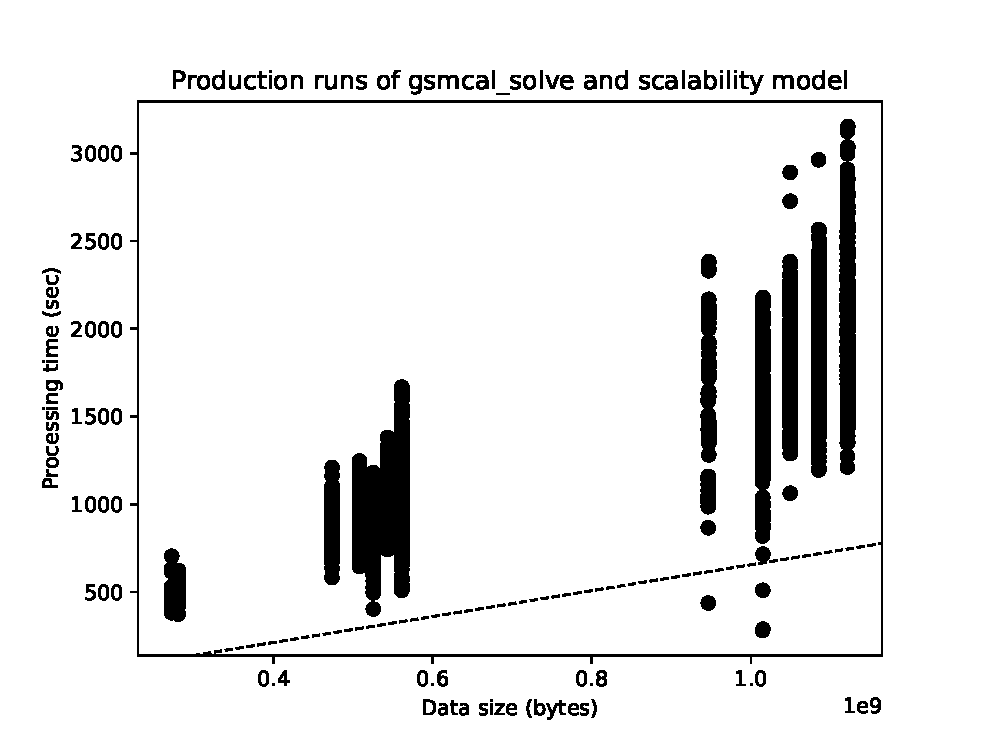
\includegraphics[width=0.95\linewidth]{ch6/figures/gsmcal_solve_size_prod.eps}
      \caption{The scalability model for processing data through the {\fontfamily{qcr}\selectfont gsmcal\_solve} step, shown in a dashed line. The scatter plot shows the performance for production runs of this step between July 2018 and January 2019. The two large clusters are for data products that are 1.0 and 2.0 GB respectively. }
	\label{fig:ch6_prod_gsmcal_times}
\end{figure}


\subsection{Complete Scalability Model}
To incorporate all our data into a complete model, we consider the slowdown of each parameter as a multiplier to the time taken to process our base run. We incorporate the models for each parameter above for the model of the run time. We add the transfer and queuing time to the processing time to obtain a final function of all our parameters. We can use this function to predict the processing time for an arbitrary data set. 

The final performance model for the slowest steps, {\fontfamily{qcr}\selectfont gsmcal\_solve}, {\fontfamily{qcr}\selectfont dpppconcat}  and {\fontfamily{qcr}\selectfont predict\_ateam} are in Equation \ref{eq:ch6_final_models}. 

\begin{equ*}[!t]
\normalsize
\begin{subequations}

\begin{equation}
 \begin{split}
   t_{infrastructure} & = \begin{cases}
        49.3\cdot\mathcal{N}+ 120 &|\mathcal{N}\leq4\\
        726\cdot\mathcal{N}-3071 & |\mathcal{N}>4
       \end{cases} \\
       & + 2 \cdot 0.056\cdot \mathcal{S}^{2.336} 
       \end{split}
 \end{equation}
     
\begin{equation}
    \begin{split}
   t_{gsmcal\_solve} & = t_{infrastructure} \\
       & + [3566\cdot \frac{1}{3.012}\mathcal{F}^{-0.854} \cdot (0.1412+\frac{0.8589}{\mathcal{N}}) ]  \cdot
          \begin{cases} 
             7.38\cdot10^{-7}\mathcal{S} | \mathcal{S}\leq16\\
             1.04\cdot10^{-6}\mathcal{S} | \mathcal{S}>16 
          \end{cases}\\
       \end{split}
 \label{eq:ch6_full_model_gsmcal}
 \end{equation}
 
 \begin{equation}
 \begin{split}
 t_{dpppconcat} &= t_{infrastructure} \\
       & + 3.51\times10^{-8}\mathcal{S}+4.20\times10^1
       \end{split}
       \label{eq:ch6_full_model_dppconcat}
 \end{equation}
 
  \begin{equation}
   \begin{split}
    t_{predict\_ateam}  &= t_{infrastructure} \\
       & + 5.19\times10^{-8}\mathcal{S}+4.20\times10^1 
       \end{split}\label{eq:ch6_full_model_predict_ateam}
  \end{equation}
\end{subequations}

\caption{Model of the total time of the most computationally expensive steps for the parameters $\mathcal{N}$, Number of CPUs; $\mathcal{S}$, Size of data in bytes and $\mathcal{F}$, cutoff calibration model flux in Jansky. These models include processing times, as well as infrastructure overheads. As the model for the queuing, downloading and uploading time does not change for different processing steps, we decide to keep it separate for clarity. The complete scalability models for the rest of the steps can be derived similarly, however are omitted here as they consist of the minority of processing time for LOFAR DI processing.  }
\label{eq:ch6_final_models}
\end{equ*}
